\section{Advective Transport: Considering Soil And Foundation Type}

The modeling in Chapter \ref{chp:preferential_pathways} help explain why building pressurization was much more strongly associated before the closing of the preferential pathway.
The preferential pathway lead to advective transport to be the dominant transport mechanism for entry of contaminant vapors through the foundation crack.
This finding has wider implications on our understanding of the entry mechanics of VI.\par

It is commonly assumed that advective transport dominates in the near-foundation region and through breaches in the foundation itself, but our modeling shows that this was only possible because:
\begin{enumerate}
  \item The preferential pathway supplied a source from where air could readily be drawn.
  \item The permeable gravel sub-base acted as a communication medium between the preferential air source and the building.
\end{enumerate}
In other words, for advective transport to dominate through foundation cracks, some site-specific features were required, and the soil itself presents too much resistance to air flow for this to be possible.\par

Only one soil type was explored in the modeling work in Chapter \ref{chp:preferential_pathways} - sandy clay, which is itself a relatively impermeable soil, and other soil type should be considered.
Furthermore, our modeled house featured a basement, and in such a scenario, the atmosphere is relatively far removed from the foundation crack, and therefore, a slab-on-grade type of foundation should also be considered.\par

The effect of different soil and foundation types is investigated using the model introduced in Chapter \ref{chp:methods}; the only difference is that we change the soil type and depth of the foundation.
We consider 12 of the soil types studied by the EPA (see Table \ref{tbl:soils}) and for each of these we consider a basement and a slab-on-grade case respectively.
The basement and slab-on-grade cases are defined by the bottom of foundation slab located at \SI{1}{\metre} and \SI{15}{\centi\metre} bgs respectively.
To building is assumed to be depressurized at $p_{in} = \SI{-15}{\pascal}$, a value much greater than "normal", to enhance the advective potential.
The analysis in Chapter \ref{chp:preferential_pathways} showed that a gravel sub-base layer, absent a preferential air source, was virtually indistinguishable from the cases where there was no gravel sub-base layer, thus such a feature will not be included in the model.\par

\begin{figure}[htb!]
  \centering
  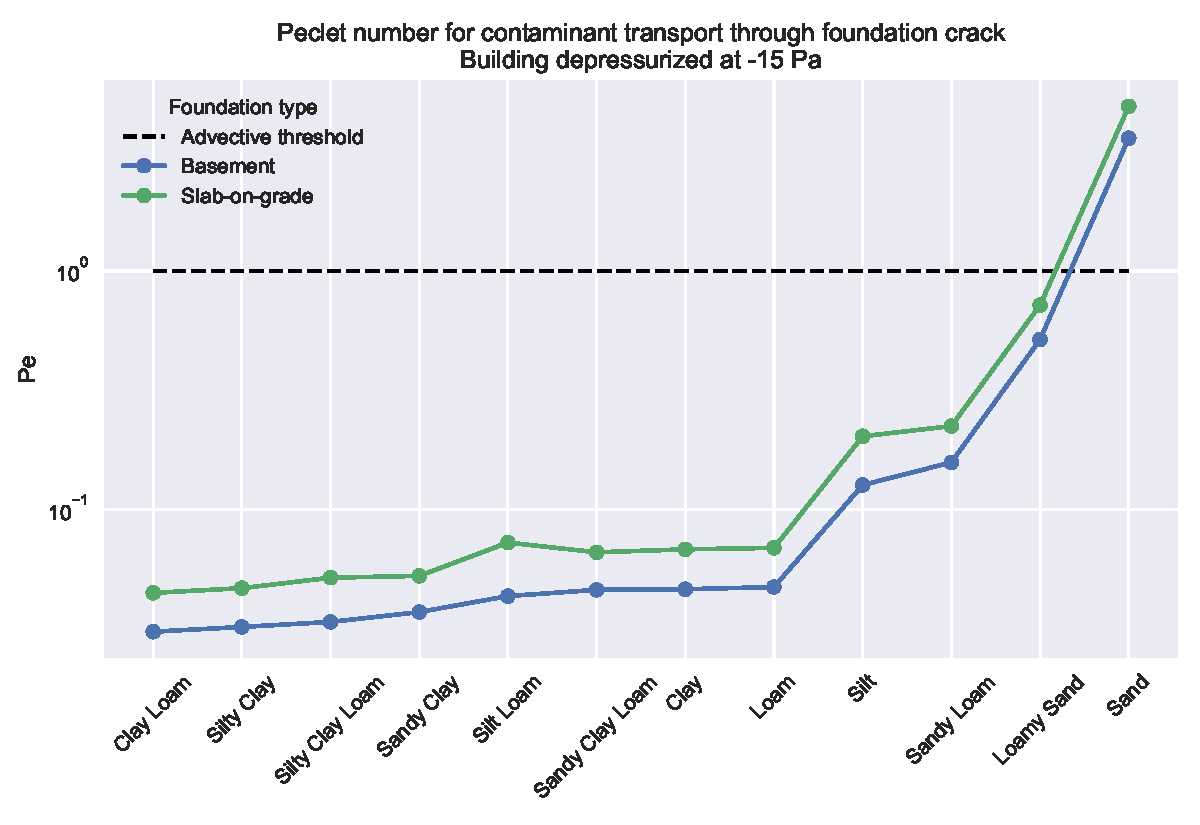
\includegraphics[width=\textwidth]{peclet_cases.pdf}
  \caption{Predicted effect of soil and foundation type on the Péclet number of transport through the foundation crack. We consider the 12 different soils studied by the EPA (see Table), and for each of these we consider a house featuring a basement and a slab-on-grade house. The foundation slab is assumed to be \SI{15}{\centi\metre} thick. In the basement case, the bottom of the foundation slab is assumed to be \SI{1}{\metre} bgs and \SI{15}{\centi\metre} bgs in the slab-on-grade case. The modeled building is assumed to be depressurized at \SI{-15}{\pascal}. The threshold where advective transport begins to overtake diffusive transport, i.e $\mathrm{Pe}=1$, is marked by the dashed line.}
  \label{fig:peclet_soil_foundation_type}
\end{figure}

The result of these model cases can be seen in Figure \ref{fig:peclet_soil_foundation_type}.
This shows that for most soil types, irrespective if a building has a basement or a slab-on-grade foundation, the Péclet number across the foundation slab is not sufficiently high for advection to the dominant transport mechanism; most soils are too impermeable for sufficient airflow to be pulled into the building via the subsurface.
Sites characterized by sand soil are an exception to this, which are permeable enough to sustain such airflows.
An example of such a site is a site at North Island Naval Air Station in San Diego, California, which featured sandy soil, and there indoor contaminant concentration and building pressurization was highly correlated\cite{hosangadi_high-frequency_2017}.\par

This indicates that for many sites characterized by other soil types, significant advective transport of contaminant vapors into the building are likely to occur through some preferential air source.
It is important to note however, that this is not limited to the sort of preferential pathways we have studied in this work, but such a phenomena could conceivably arise from a wide range of circumstances.\par
